\documentclass{article}
\usepackage{graphicx} % Required for inserting images
\usepackage{amsmath}
\usepackage{amsfonts}
\usepackage{tikz}
\usepackage{venndiagram}

\def\firstcircle{(90:1.75cm) circle (2.5cm)}
\def\secondcircle{(210:1.75cm) circle (2.5cm)}
\def\thirdcircle{(330:1.75cm) circle (2.5cm)}

\tikzset{venn circle/.style={draw=gray,text opacity=1,fill opacity=0.25,circle,minimum width=10cm,fill=#1,line width=2pt}}
\tikzset{label/.style={text width=1.5cm,font=\large\sffamily}}

\title{Introducci\'on al lenguaje de las matem\'aticas}
\author{Roberto G. Fernández}
\date{Febrero 2024}

\begin{document}

\maketitle


\section{Conjuntos num\'ericos}
\subsection{Teor\'ia de conjuntos}

\subsubsection{Conceptos b\'asicos}
Un conjunto es una colecci\'on de objetos, y est\'a bien
definido si se sabe si un determinado elemento pertenece o no
a \'el.

Llamaremos elemento a cada uno de los objetos que forman parte de un conjunto. Usualmente se representan con una letra min\'uscula, en tanto que los conjuntos, con una may\'uscula.
Para indicar que un elemento x pertenece a un conjunto A, escribimos:

\begin{equation}
x \in A
\end{equation}

La negaci\'on de \begin{math}x \in A\end{math} se escribe:

\begin{equation}
x \notin A
\end{equation}

Dos conjuntos especiales son:
\begin{itemize}
  \item El conjunto universal, que representaremos con la letra U, es el conjunto de todas las cosas sobre las que estemos tratando.
  \item El conjunto vac\'io, que se denota \begin{math}\emptyset\end{math}, que no tiene elementos.
\end{itemize}

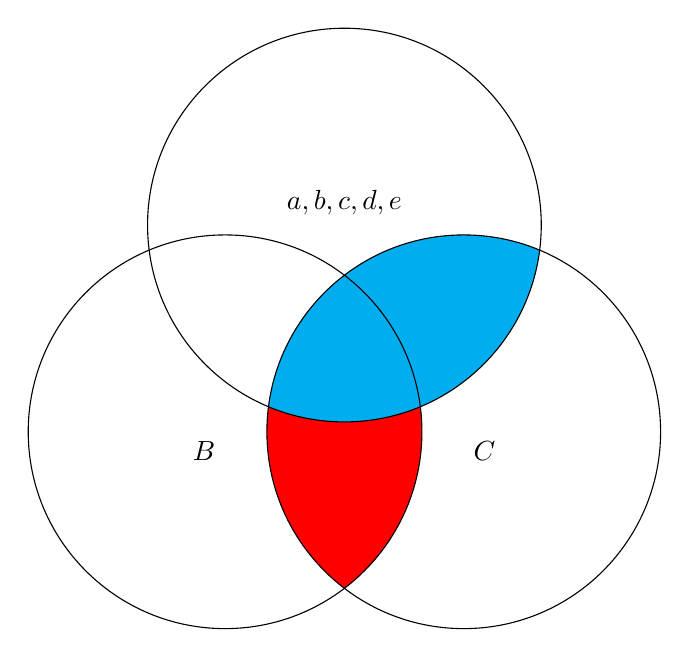
\begin{tikzpicture}
  \begin{scope}
    \clip \secondcircle;
    \fill[red] \thirdcircle;
  \end{scope}
  \begin{scope}
    \clip \firstcircle;
    \fill[cyan] \thirdcircle;
  \end{scope}
  \draw \firstcircle node[text=black,above] {$a,b,c,d,e$};
  \draw \secondcircle node [text=black,below left] {$B$};
  \draw \thirdcircle node [text=black,below right] {$C$};
\end{tikzpicture}

\begin{venndiagram3sets}[radius=5cm,overlap=3cm,
                         tikzoptions={text opacity=1,fill opacity=0.25},
                         labelOnlyBC={\begin{tabular}{l} text1,\\text2,\\text3,\\text4 \end{tabular}}]
   \fillBCapCNotA 
\end{venndiagram3sets}


\end{document}